\documentclass[11pt]{article}

%% MinionPro fonts 
%\usepackage[lf]{MinionPro}
%\usepackage{MnSymbol}
\usepackage{microtype}

%% Margins
\usepackage{geometry}
\geometry{verbose,letterpaper,tmargin=1in,bmargin=1in,lmargin=1in,rmargin=1in}

%% Other packages
\usepackage{amsmath}
\usepackage{amsthm}
\usepackage[shortlabels]{enumitem}
\usepackage{titlesec}
\usepackage{soul}
\usepackage{tikz}
\usepackage{mathtools}
\usepackage{pgfplots}
\usepackage{tikz-3dplot}
\usepackage{algorithmic}
\usepackage[export]{adjustbox}
\usepackage{tcolorbox}
\usepackage{mathrsfs}
\usepackage{multicol}
\usepackage{framed}

%% Paragraph style settings
\setlength{\parskip}{\medskipamount}
\setlength{\parindent}{0pt}

%% Change itemize bullets
\renewcommand{\labelitemi}{$\bullet$}
\renewcommand{\labelitemii}{$\circ$}
\renewcommand{\labelitemiii}{$\diamond$}
\renewcommand{\labelitemiv}{$\cdot$}

%% Colors
\definecolor{rred}{RGB}{204,0,0}
\definecolor{ggreen}{RGB}{0,145,0}
\definecolor{yyellow}{RGB}{255,185,0}
\definecolor{bblue}{rgb}{0.2,0.2,0.7}
\definecolor{ggray}{RGB}{190,190,190}
\definecolor{ppurple}{RGB}{160,32,240}
\definecolor{oorange}{RGB}{255,165,0}

%% Shrink section fonts
\titleformat*{\section}{\normalsize\bf}
\titleformat*{\subsection}{\normalsize\bf}
\titleformat*{\subsubsection}{\normalsize\it}

% %% Compress the spacing around section titles
\titlespacing*{\section}{0pt}{1.5ex}{0.75ex}
\titlespacing*{\subsection}{0pt}{1ex}{0.5ex}
\titlespacing*{\subsubsection}{0pt}{1ex}{0.5ex}

%% amsthm settings
\theoremstyle{definition}
\newtheorem{problem}{Problem}
\newtheorem{example}{Example}
\newtheorem*{theorem}{Theorem}
\newtheorem*{bigthm}{Big Theorem}
\newtheorem*{biggerthm}{Bigger Theorem}
\newtheorem*{bigcor1}{Big Corollary 1}
\newtheorem*{bigcor2}{Big Corollary 2}

%% tikz settings
\usetikzlibrary{calc}
\usetikzlibrary{patterns}
\usetikzlibrary{decorations}
\usepgfplotslibrary{polar}

%% algorithmic setup
\algsetup{linenodelimiter=}
\renewcommand{\algorithmiccomment}[1]{\quad// #1}
\renewcommand{\algorithmicrequire}{\emph{Input:}}
\renewcommand{\algorithmicensure}{\emph{Output:}}

%% Answer box macros
%% \answerbox{alignment}{width}{height}
\newcommand{\answerbox}[3]{%
  \fbox{%
    \begin{minipage}[#1]{#2}
      \hfill\vspace{#3}
    \end{minipage}
  }
}

%% \answerboxfull{alignment}{height}
\newcommand{\answerboxfull}[2]{%
  \answerbox{#1}{6.38in}{#2} 
}

%% \answerboxone{alignment}{height} -- for first-level bullet
\newcommand{\answerboxone}[2]{%
  \answerbox{#1}{6.0in}{#2} 
}

%% \answerboxtwo{alignment}{height} -- for second-level bullet
\newcommand{\answerboxtwo}[2]{%
  \answerbox{#1}{5.8in}{#2}
}

%% special boxes
\newcommand{\wordbox}{\answerbox{c}{1.2in}{1cm}}
\newcommand{\catbox}{\answerbox{c}{.5in}{1cm}}
\newcommand{\letterbox}{\answerbox{c}{.7cm}{1cm}}

%% Miscellaneous macros
\newcommand{\tstack}[1]{\begin{multlined}[t] #1 \end{multlined}}
\newcommand{\cstack}[1]{\begin{multlined}[c] #1 \end{multlined}}
\newcommand{\ccite}[1]{\only<presentation>{{\scriptsize\color{gray} #1}}\only<article>{{\small [#1]}}}
\newcommand{\grad}{\nabla}
\newcommand{\ra}{\ensuremath{\rightarrow}~}
\newcommand{\maximize}{\text{maximize}}
\newcommand{\minimize}{\text{minimize}}
\newcommand{\subjectto}{\text{subject to}}
\newcommand{\trans}{\mathsf{T}}
\newcommand{\bb}{\mathbf{b}}
\newcommand{\bx}{\mathbf{x}}
\newcommand{\bc}{\mathbf{c}}
\newcommand{\bd}{\mathbf{d}}

%% LP format
%    \begin{align*}
%      \maximize \quad & \mathbf{c}^{\trans} \mathbf{x}\\
%      \subjectto \quad & A \mathbf{x} = \mathbf{b}\\
%                       & \mathbf{x} \ge \mathbf{0}
%    \end{align*}

%Space between rows:
%\def\arraystretch{2.2}
%
%Space between columns:
%\arraycolsep=1.4pt


%% Redefine maketitle
\makeatletter
\renewcommand{\maketitle}{
  \noindent SA405 -- AMP \hfill Rader \S 4.2 \\

  \begin{center}\Large{\textbf{\@title}}\end{center}
}
\makeatother

%% ----- Begin document ----- %%
\begin{document}
  
\title{Lesson 10.  Facility Location}

\maketitle

%%%
\section{Facility Location Introduction}

The \textbf{facility location} problem is another famous OR problem which is very applied for industry/military applications. In this lesson, we will look at 3 different types of formulations of this problem.


In these problems, the \textbf{input data} is...
\begin{itemize}
\item  a network of ``customers'' (demand nodes),
\item  a set of \emph{possible} ``facilities'' (supply nodes),
\item  a set of edges between customers and facilities that \emph{could} serve them
\item  distances on the edges (which could represent distance, time, cost, or some combination of these factors)
\end{itemize} 


The \textbf{goal} is to choose a set of supply facilities to serve the customers' demand based on some metric.
\begin{itemize}
\item For example: minimize the number of supply facilities opened while requiring that all customers are served.  
\item The different problem types result from varied metrics and/or requirements.
\item  Real world problems of this type include locating 
\begin{itemize}
\item military installations, 
\item fire/police stations, 
\item cell phone towers, 
\item retail distribution centers and stores, 
\item schools,
\item vaccine clinics.
\end{itemize}
\end{itemize}

%\bigskip
%\begin{tcolorbox}
%\renewcommand\labelitemi{$\circ$}
%\textbf{Basic Facility Location Assumptions:}
%\begin{itemize}
%	\item \textbf{Simple graph $G = (V, E)$}
%	\item Demand locations, $I \subseteq V$, are given
%	\item \emph{Possible} supply facility locations, $J \subseteq V$, are given
%	\begin{itemize}
%	\item[--] ($I$ and $J$ may have common nodes)
%	\end{itemize}
%	\item Edge $(i,j) \in E$ indicates that it is possible for a customer at $i$ to be supplied by a facility at $j$ (or customer at $j$ may be served by facility at $i$)
%	\begin{itemize}
%	\item[--] There is a ``distance'' $d_{c,s}$ assigned to every edge $(i,j) \in E$
%	\end{itemize}
%\end{itemize}
%\end{tcolorbox}

\newpage
\section{\emph{General} Facility Location Problems}
%\begin{center}
%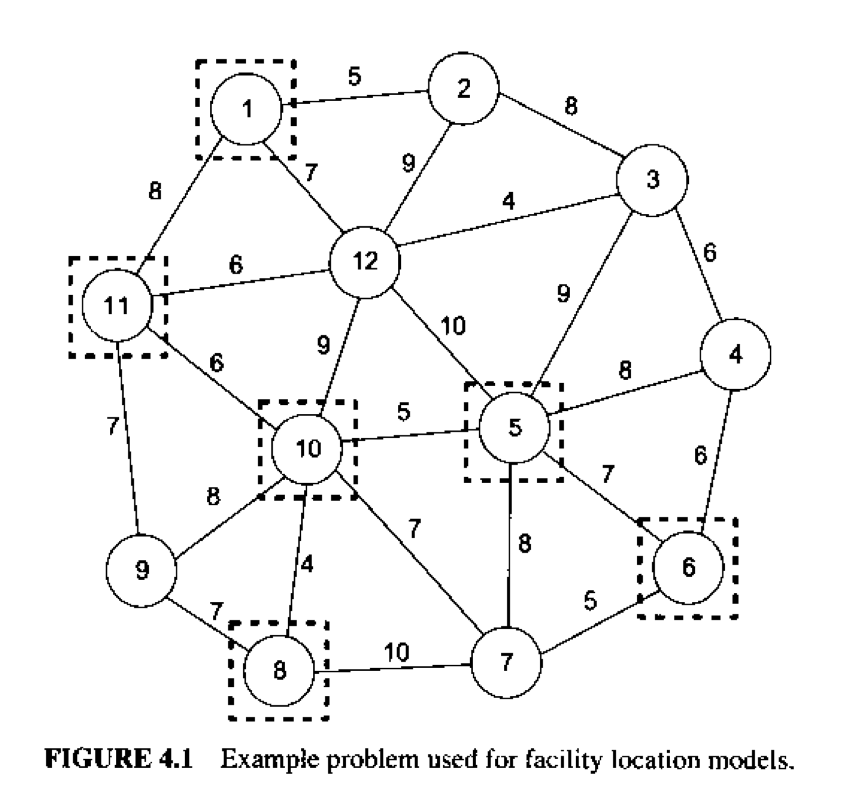
\includegraphics[width = 0.6\textwidth]{facloc}
%\end{center}

\bigskip
\begin{tcolorbox}
\textbf{Goal:} Choose a set of supply facilities to meet customer demand according to some metric.  
\end{tcolorbox}

\textbf{Notation:}

Sets: 
\begin{itemize}
\item[]
 C = set of customer nodes 
\item[]
S = set of possible supply nodes 
\item[]
E = edges $(c,s)$ connecting a customer $c$ with a supply facility $s$ that \emph{could} serve the customer
\end{itemize}

Parameters: 
\begin{itemize}
\item[]
 $d_{c,s} =$ distance (or cost or time) between customer $c$ and supply location $s$, for $(c,s) \in E$
 \item[]
 $h_c =$ demand of customer $c$, for $c \in C$
\end{itemize}


\smallskip
Decision Variables: 
\begin{itemize}
\item[] 
\def\arraystretch{1.8} 
$x_s = ~\left\{ 
\begin{array}{ll} 
1 \text{ if } ~\answerbox{c}{3in}{.7cm} \\ 
0 \text{ otherwise } 
\end{array} \right. $
, for all $s \in S$
\end{itemize}

\vspace{0.5cm}
\begin{problem} We will use the network and data on the following page for all of our example problems.
\begin{enumerate}[(a)] 
\item \emph{All} vertices represent customers.  \emph{Boxed} vertices represent possible supply locations. Use set notation to list the elements of the sets $C$ and $S$.  

\vspace{1.5cm}

\item The distance between a customer $c$ and a supplier $s$ is the length of the shortest path between them.
Find $d_{1,1}$, $d_{4,1}$, and $d_{8,5}$.  (Note that the ``edges'' in the model do not correspond directly to the edges in the graph.)

\vspace{1.5cm}

\item How should the columns and rows in the distance matrix be labeled?  Do your answers in part (a) agree with the corresponding values in the distance matrix?  

\vfill
\end{enumerate}
\end{problem}

%%%%
\newpage
DATA for FACILITY LOCATION EXAMPLES:

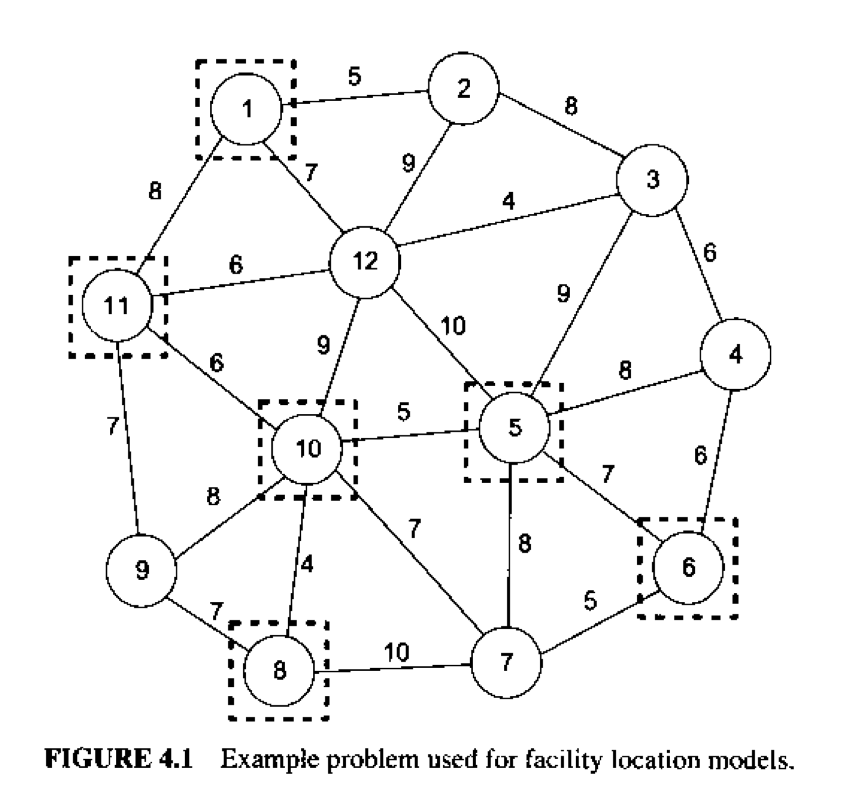
\includegraphics[width = 0.7\textwidth]{facloc}

\vfill
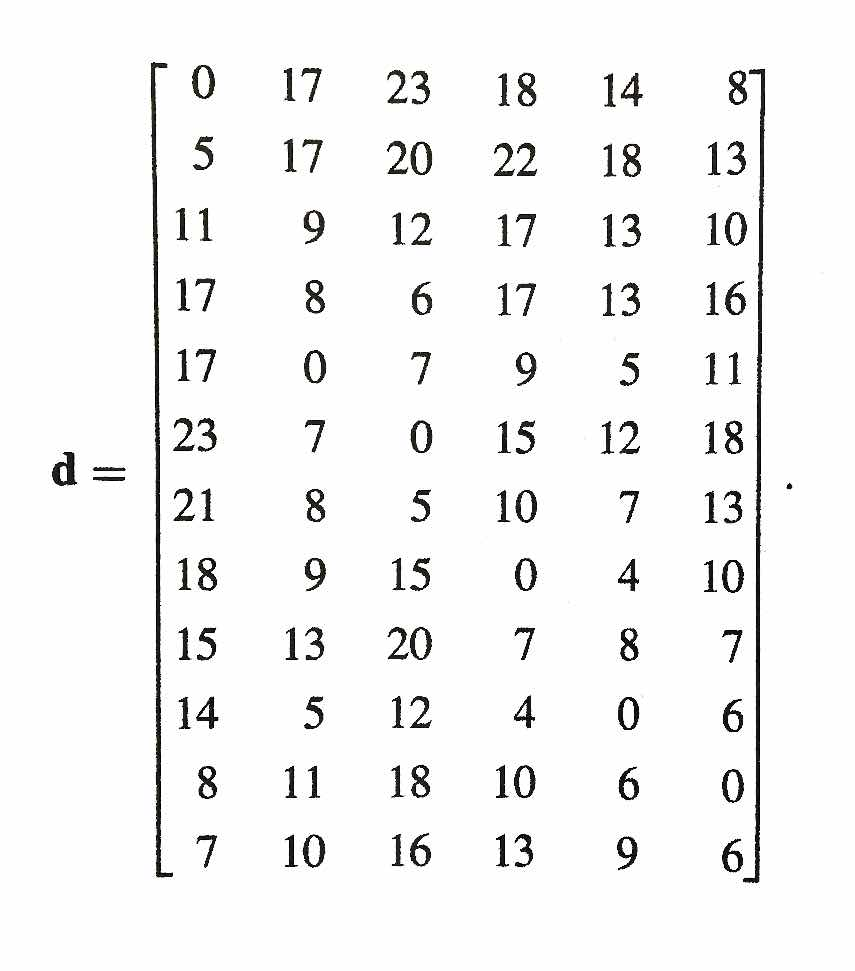
\includegraphics[width = 0.4\textwidth]{Distances}

\vfill
$\textbf{h} = (100,~ 90,~ 110,~ 120,~ 80,~ 100,~ 95, ~75,~ 110,~ 90, ~120, ~85).$

\vfill


%%%
\newpage

\vspace{1in}
\section{Simplest Facility Location Model: \emph{Set Covering}}

Given a set of potential facilities to open, open the fewest number of facilities such that each customer is ``covered'' by at least one facility.

\begin{problem}
Find the minimum number of facilities required to serve all customers.  A facility must be within $D = 9$ miles of a customer in order to serve the customer.

\begin{enumerate}[(a)]
\item We define a new set for each customer, referred to as the neighborhood of customer $c$, $N_c$. $N_c$ is the set of facilities that can cover customer $c$:  
\[  N_c = \left\{s \in S: ~\wordbox~\right\}, \text{ for all } c \in C.  \]
\item Complete the missing neighborhoods.   

\def\arraystretch{2.2}
\begin{multicols}{2}
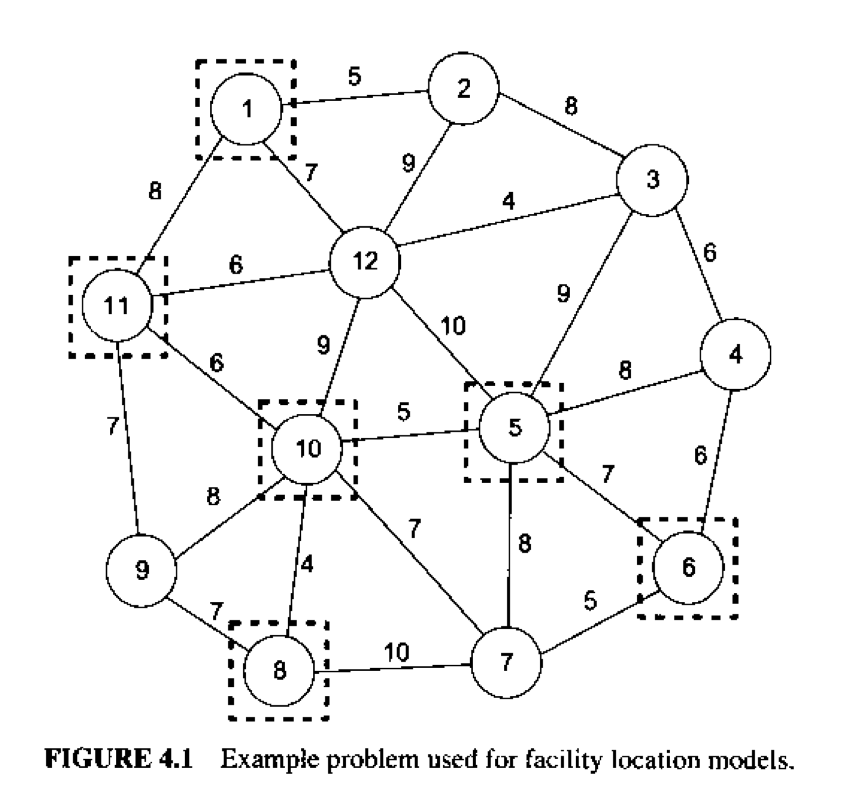
\includegraphics[width = 0.4\textwidth]{facloc}
$
\begin{array}{ll}
N_1 = \{1, 11\} \hspace{2cm} & N_7 = \{5, 6, 10\} \\
N_2 = \{1\} & N_8 = \catbox \\
N_3 = \catbox  & N_9 = \{8,10,11\} \\
N_4 = \{5,6\} & N_{10} = \catbox \\
N_5 = \{5,6,8,10\} & N_{11} = \{1,10,11\} \\
N_6 = \{5,6\} & N_{12}= \catbox \\
\end{array}
$
\end{multicols}
\item Write an abbreviated version of the concrete model using the $x_s$ variables defined above.


\newpage

\item Using the sets and variables defined below, complete the parameterized set covering facility location model.

\textbf{\underline{Sets}}

Let $S$ be the set of possible supply locations\\
Let $C$ be the set of all customers \\
Let $N_c$ be the neighborhood of customer $c$ for all $c \in C$


\textbf{\underline{Variables}}

Let $x_s = 1$ if a facility is placed at location $s$ and 0 otherwise for all $s \in S$.
\end{enumerate}
\end{problem}

\vfill

What's the drawback of this model? In other words, what makes this problem unrealistic? \vspace{1in}



%%%%
\newpage
\section{\emph{Maximal Covering} Location Problem}
The \textbf{maximal covering location problem}: Given $p$ facilities to open, maximize the customer demand that is covered.  (A customer, $c$, can only be covered by a supply facility, $s$, in its neighborhood: $s \in N_c$.)

\begin{center}
\noindent{\textbf{Maximal covering facility location model}}
\end{center}

\textbf{
\emph{New} Parameters: }
\begin{itemize}
\item[] $h_c = $ the demand at customer $c$, for all $c \in C$
\item[]  $p = $ the number of facilities to open
\end{itemize}
\textbf{\emph{New} Decision Variables: }
\begin{itemize}
\item[] \def\arraystretch{1.8} $y_c = ~\left\{ \begin{array}{ll} 1 \text{ if }~\answerbox{c}{3in}{.7cm} \\ 0 \text{ otherwise } \end{array} \right. $
, for all $c \in C$
\end{itemize}

\begin{problem}
Assuming that 2 facilities can be opened, write a concrete mode for the maximal covering facility location using the data from page 3.
\end{problem}

\newpage

\begin{problem}
Write the parameterized version of the maximal covering facility location model.
\end{problem}


%%%%
\newpage
\subsection{Example:  Maximal Covering Facility Location Problem}

\begin{problem}
Suppose that we can only afford to build and maintain $p = 2$ facilities, and the demand values for the customers (in order) are 
\[
\textbf{h} = (100, 90, 110, 120, 80, 100, 95, 75, 110, 90, 120, 85).
\]
\end{problem}

\begin{enumerate}[(a)]
\item The optimal solution is to choose facilities 5 and 11.  List the values of the decision variables $x_s$ and $y_c$ in the optimal solution.  Illustrate the solution on the graph of the network.

\hfill 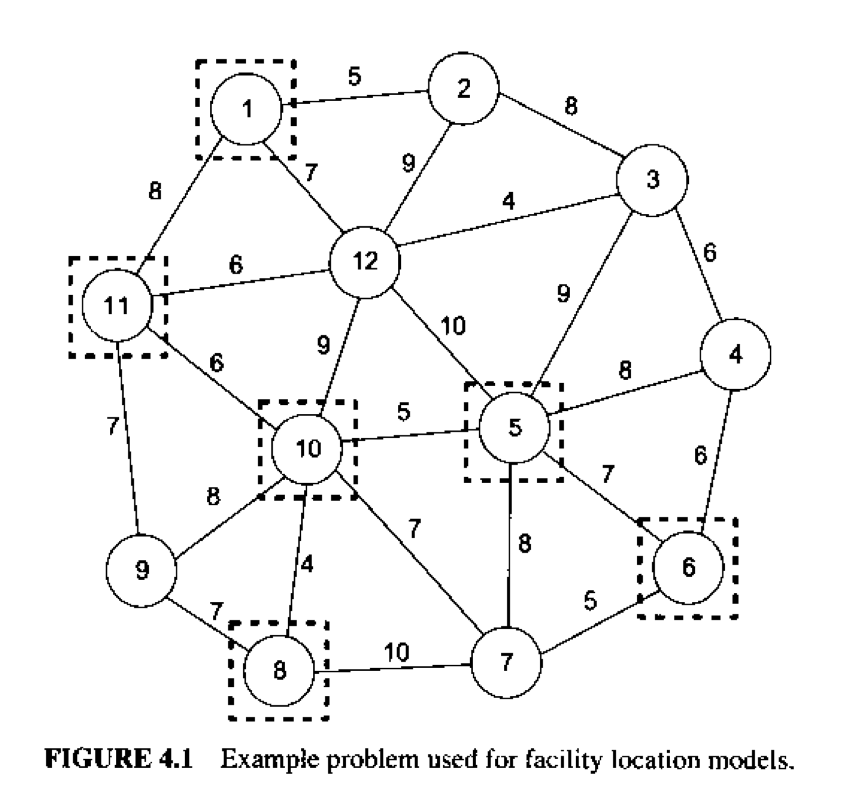
\includegraphics[width = 0.5\textwidth]{facloc}

\item Find the optimal objective function value.  What does it mean? \vspace{2cm}
	

\item Suppose we allow $p = 3$
\begin{enumerate}[i]
\item Which new facility would we open to cover the most demand?

\vfill 
\item What would be our new objective function value?

\vfill 


\end{enumerate}
\end{enumerate}

\newpage

%%%%
\section{\emph{$p$-Center} Facility Location Problem:  Minimize Maximum Distance}

Goal of the \textbf{$p$-center problem}: Choose $p$ supply facilities to open in order to minimize the maximum distance between any customer and the supply facility that serves it.

\begin{problem} 
Complete the $p$-center facility location formulation below by filling in the missing constraints and descriptions.

\begin{center}
\noindent{\textbf{$p$-center facility location model}}
\end{center}


\textbf{\emph{New} Decision Variables: }
\begin{itemize}
\item[] \def\arraystretch{1.8} $z_{c,s} = ~\left\{ \begin{array}{ll} 1 \text{ if} ~\answerbox{c}{3in}{.7cm}  
\\ 0 \text{ otherwise } \end{array} \right. $
, for all $c \in C,~ s \in S$
\item[] $W = $ the maximum distance between a customer and the facility chosen to serve it
\end{itemize}
\emph{Notice that by the way $z_{c,s}$ is defined, we assume that each customer could be served by any supplier.}
%\vspace{-.2ztcm}


\medskip

\noindent \textbf{Objective and constraint descriptions:}

(1) and (2) \answerbox{c}{13.9cm}{3cm}
% This is a mini-max formulation.  (2) says that $W$ is no less than the distance between any customer and the facility that serves it.  The downward pressure of (1) ensures that $W$ is exactly the maximum distance between any customer and the facility that serves it.

(3) %\answerboxone{c}{1.7cm}
 Exactly $p$ facilities are opened

(4) \answerboxone{c}{1cm}
% Customer $c$ is assigned to exactly one facility

(5) %\answerboxone{c}{1.7cm}
 Customer $c$ cannot be assigned to a facility that is not open

\vspace{-.5cm}
    \begin{align}
      \minimize \quad & W  \\
      \subjectto \quad 
 					   & \sum_{s \in S} d_{c,s}z_{c,s} \leq W, \text{ for } c \in C \\
%      	                              & \sum_{s \in S} x_s = p \\
 					   & \answerbox{c}{8cm}{1cm} \\
 				          & \sum_{s \in S} z_{c,s} = 1, \text{ for } c \in C \\
 %					  & z_{c,s} \leq x_s, \text{ for } c \in C,~s \in S \\
 					   & \answerbox{c}{8cm}{1cm} \\
                       & x_s \in \{0,1\}, \text{ for } s \in S \nonumber\\
                       & z_{c,s} \in \{0,1\}, \text{ for } c \in C, ~s \in S \nonumber
    \end{align}



\end{problem}

%%%%
\newpage

\subsection{Example:  $p$-Center Facility Location Problem}

\begin{problem}
Assume the same network, distances, and demand values that we have already been using.  We wish to find the
$p=2$ facilities that can serve all of the customers so that the maximum distance between a customer and the facility it is served by is minimized.
\end{problem}

\begin{enumerate}[(a)]
\item Again, the optimal solution is to choose facilities 5 and 11. Facility 5 serves the customers 3, 4, 5, 6, 7, and 8.  Facility 11 serves the rest.  Write the values of the decision variables for this optimal solution and draw the solution on the network.

\hspace{-3cm} 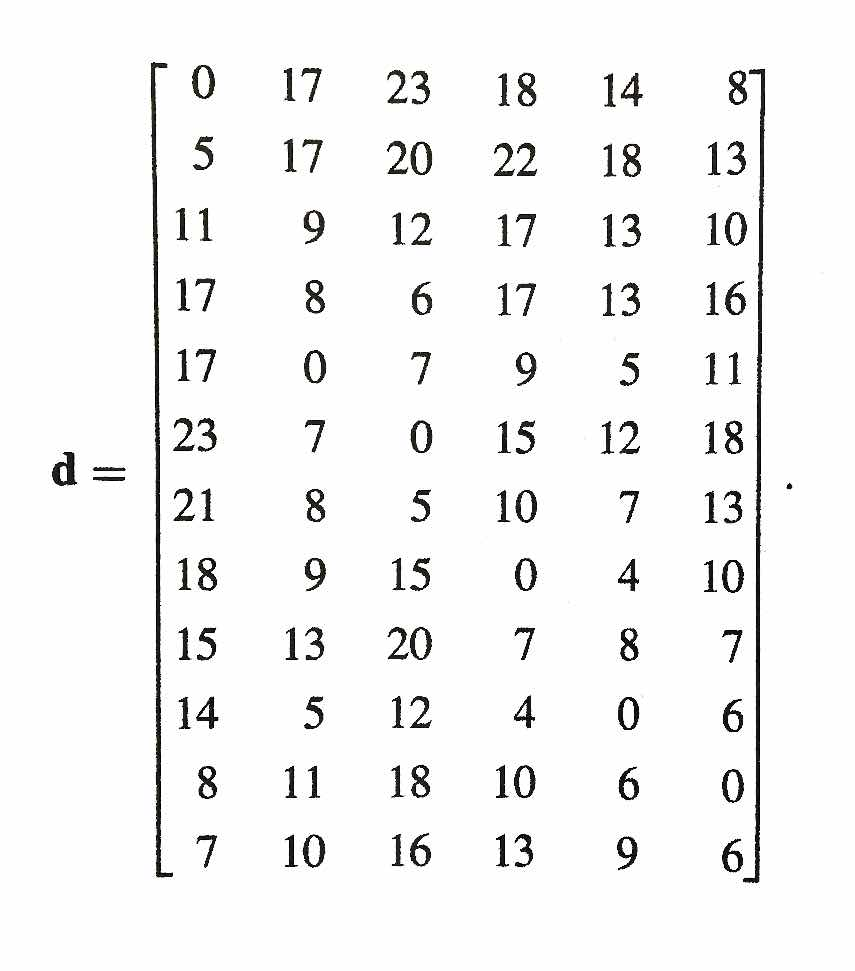
\includegraphics[width = 0.3\textwidth]{Distances} 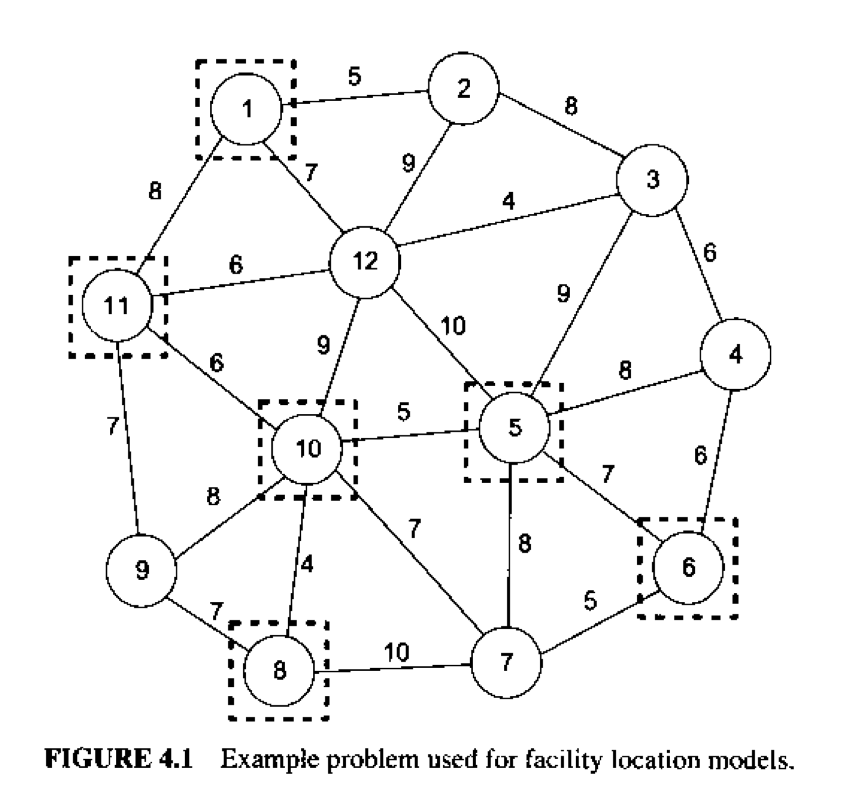
\includegraphics[width = 0.4\textwidth]{facloc} 
\phantom{\answerbox{b}{6.2cm}{5.8cm}}

\item Find the optimal objective function value.  What does it mean?

\vspace{1.7cm}
\item Write concrete versions of the following:
\begin{enumerate}[i]
\item constraint (2) for customers 2 and 3:

\vspace{2.2cm}


\item constraint (4) for customer 2:

\vspace{1cm}

\item constraints (5) for supplier 5 and all of its potential customers:

\vspace{1.9cm}
\end{enumerate}
\end{enumerate}

%%%%
\newpage


\section{Summary}
We discuss 3 common types of facility location models. These models, and their goals were:
\begin{itemize}
\item \phantom{hi} 
\item \phantom{hi} \vspace{1in}
\item \phantom{hi} \vspace{1in}
\end{itemize}
\vspace{1in}

This is \textbf{not} an all inclusive list of models. Typically, one could use one of these as a starting point and then expand from there. Other things to model include:
	\begin{itemize}
	\item A fixed charge associated with each facility (think back to Lesson 5)
	\item Incorporating logical constraints like in Lesson 7
	\item Multiperioud facility location (can be quite difficult)
	\item Different objective functions such as:
		\begin{itemize}
		\item Minimizing the average distance traveled
		\item Minimizing a weighted distance (i.e., prioritize customers with high demand)
		\item Opening facilities based on need (i.e., some areas have a priority)
		\item etc...
		\end{itemize}
	\end{itemize}





\end{document}